% Choose one to switch between slides and handout
\documentclass[]{beamer}
%\documentclass[handout]{beamer}

% Video Meta Data
\title{Bitcoin, Blockchain and Cryptoassets}
\subtitle{Monetary Theory Basics}
\author{Prof. Dr. Fabian Schär}
\institute{University of Basel}

% Config File
% Packages
\usepackage[utf8]{inputenc}
\usepackage{hyperref}
\usepackage{gitinfo2}
\usepackage{tikz}
\usepackage{amsmath}
\usepackage{bibentry}
\usepackage{xcolor}
\usepackage{colortbl} % Add colour to LaTeX tables
\usepackage{caption}
\usepackage[export]{adjustbox}
\usepackage{pgfplots} \pgfplotsset{compat = 1.17}

% Color Options
\definecolor{highlight}{rgb}{0.65,0.84,0.82}
\definecolor{focus}{rgb}{0.72, 0, 0}

% Beamer Template Options
\beamertemplatenavigationsymbolsempty
\setbeamertemplate{footline}[frame number]
\setbeamercolor{structure}{fg=black}
\setbeamercolor{footline}{fg=black}
\setbeamercolor{title}{fg=black}
\setbeamercolor{frametitle}{fg=black}
\setbeamercolor{item}{fg=black}
\setbeamercolor{}{fg=black}
\setbeamercolor{bibliography item}{fg=black}
\setbeamercolor*{bibliography entry title}{fg=black}
\setbeamertemplate{items}[square]
\setbeamertemplate{enumerate items}[default]
\captionsetup[figure]{labelfont={color=black},font={color=black}}
\captionsetup[table]{labelfont={color=black},font={color=black}}

\setbeamertemplate{bibliography item}{\insertbiblabel}

% Link Icon Command
\newcommand{\link}{%
    \tikz[x=1.2ex, y=1.2ex, baseline=-0.05ex]{%
        \begin{scope}[x=1ex, y=1ex]
            \clip (-0.1,-0.1)
                --++ (-0, 1.2)
                --++ (0.6, 0)
                --++ (0, -0.6)
                --++ (0.6, 0)
                --++ (0, -1);
            \path[draw,
                line width = 0.5,
                rounded corners=0.5]
                (0,0) rectangle (1,1);
        \end{scope}
        \path[draw, line width = 0.5] (0.5, 0.5)
            -- (1, 1);
        \path[draw, line width = 0.5] (0.6, 1)
            -- (1, 1) -- (1, 0.6);
        }
    }

% Read Git Data from Github Actions Workflow
% Defaults to gitinfo2 for local builds
\IfFileExists{gitInfo.txt}
	{\input{gitInfo.txt}}
	{
		\newcommand{\gitRelease}{(Local Release)}
		\newcommand{\gitSHA}{\gitHash}
		\newcommand{\gitDate}{\gitAuthorIsoDate}
	}

% Custom Titlepage
\defbeamertemplate*{title page}{customized}[1][]
{
  \vspace{-0cm}\hfill
\includegraphics[width=2.5cm]{../config/logo_cif}
  
\includegraphics[width=1.9cm]{../config/seal_wwz}
  \\ \vspace{2em}
  \usebeamerfont{title}\textbf{\inserttitle}\par
  \usebeamerfont{title}\usebeamercolor[fg]{title}\insertsubtitle\par  \vspace{1.5em}
  \small\usebeamerfont{author}\insertauthor\par
  \usebeamerfont{author}\insertinstitute\par \vspace{2em}
  \usebeamercolor[fg]{titlegraphic}\inserttitlegraphic
    \tiny \noindent \texttt{Release Ver.: \gitRelease}\\ 
    \texttt{Version Hash: \gitSHA}\\
    \texttt{Version Date: \gitDate}\\ \vspace{1em}
  \link \href{https://github.com/cifunibas/Bitcoin-Blockchain-Cryptoassets/blob/main/slides/intro.pdf}
  {Get most recent version}\\
  \link \href{https://github.com/cifunibas/Bitcoin-Blockchain-Cryptoassets/blob/main/slides/intro.pdf}
  {Watch video lecture}\\ \vspace{1em}
  License: \texttt{Creative Commons Attribution-NonCommercial-ShareAlike 4.0 International}\\\vspace{2em}
  
\includegraphics[width = 1.2cm]{../config/license}
}

% tikzlibraries
\usetikzlibrary{decorations.pathreplacing}
\usetikzlibrary{decorations.markings}
\usetikzlibrary{positioning}

%caption font
\captionsetup{font=footnotesize}


%%%%%%%%%%%%%%%%%%%%%%%%%%%%%%%%%%%%%%%%%%%%%%
%%%%%%%%%%%%%%%%%%%%%%%%%%%%%%%%%%%%%%%%%%%%%%

\begin{document}

\thispagestyle{empty}
\begin{frame}[noframenumbering]
	\titlepage
\end{frame}

%%%
\begin{frame}{What Is Money?}
	Thought experiment: community without money
	\vspace{1.5em}
	\begin{figure}
		\begin{tikzpicture}
	% top left: smith
	\node (smith) at (-3, 2){
\includegraphics[height = 0.15\textheight]{../assets/images/agents/agent_right}};
	
	% top right: saddler
	\node (saddler) at (3, 2){
\includegraphics[height = 0.15\textheight]{../assets/images/agents/agent_left}};

	\draw[<->, very thick] (smith.east) -- (saddler.west) node[midway, above]{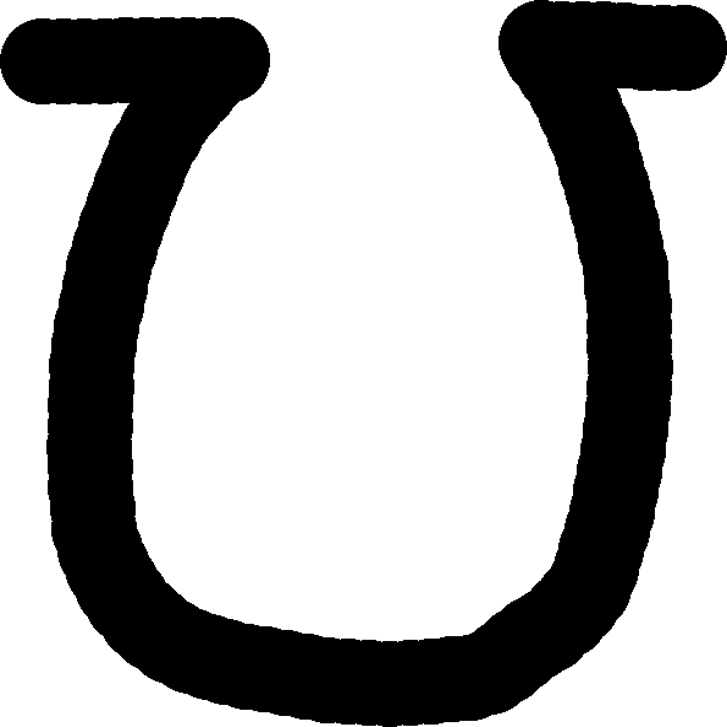
\includegraphics[height = 0.08\textheight]{../assets/images/horseshoe}} node[midway, below]{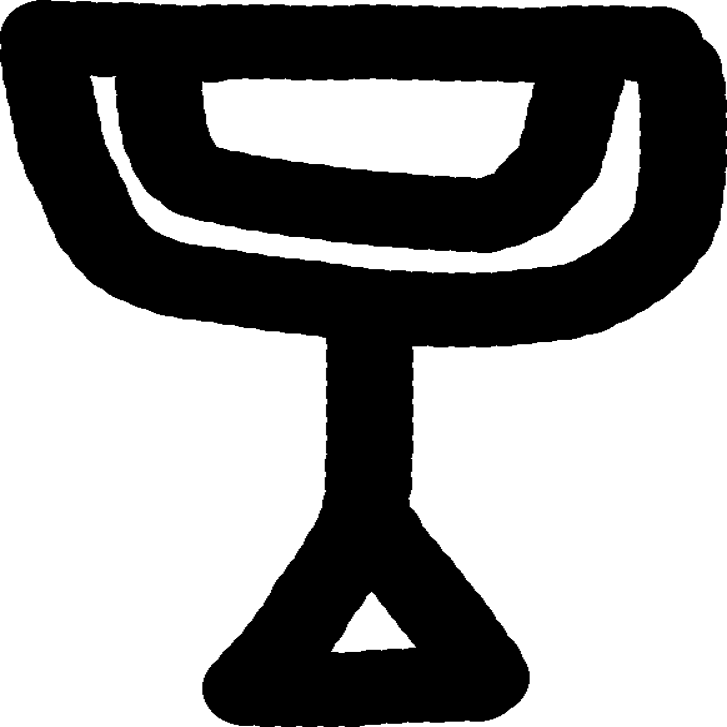
\includegraphics[height = 0.08\textheight]{../assets/images/saddle}};
	
\end{tikzpicture}
	\end{figure}
\end{frame}
%%%

%%%
\begin{frame}{The Three Basic Functions of Money}
	Money performs three basic functions:
	\begin{figure}
		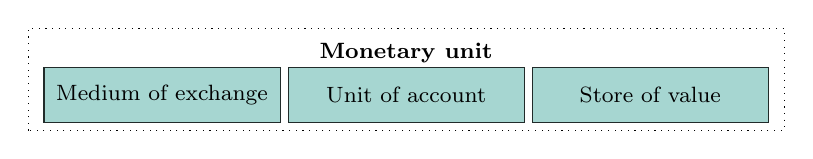
\begin{tikzpicture}
	\begin{footnotesize}
		\draw[dotted, above] (0,0) rectangle (9.6, 1.3) node[above = 3pt, midway] (Unit) {\textbf{Monetary unit}};
		\uncover<2->{\filldraw[fill = highlight, draw = highlight!20!black] (0.2, 0.1) rectangle (3.2, 0.8) node[midway] {Medium of exchange};}
		\uncover<3->{\filldraw[fill = highlight, draw = highlight!20!black] (3.3, 0.1) rectangle (6.3, 0.8) node[midway] {Unit of account};}
		\uncover<4->{\filldraw[fill = highlight, draw = highlight!20!black] (6.4, 0.1) rectangle (9.4, 0.8) node[midway] {Store of value};}
	\end{footnotesize}
\end{tikzpicture}
	\end{figure}
	\uncover<2->{\textbf{Medium of exchange:} more efficient trade and optimized allocation of goods and services.} \\
	\vspace{0.5em}
	\uncover<3->{\textbf{Unit of account:} universal reference to simplify the comparison of value between goods and services.} \\
	\vspace{0.5em}
	\uncover<4->{\textbf{Store of value:} saving.}
\end{frame}
%%%

%%%
\begin{frame}{Generally Accepted Medium of Exchange}
	Money may emerge without government intervention \cite{mengerOrigin1892}.
	\vspace{1.5em}
	\begin{figure}
		\begin{tikzpicture}
	% top left: smith
	\node (smith) at (-3, 2){
\includegraphics[height = 0.15\textheight]{../assets/images/agents/agent_right}};
	
	% top right: saddler
	\node (saddler) at (3, 2){
\includegraphics[height = 0.15\textheight]{../assets/images/agents/agent_left}};
	
	\draw[->, very thick] ([yshift = 0.15cm]smith.east) -- ([yshift = 0.15cm]saddler.west) node[midway, above]{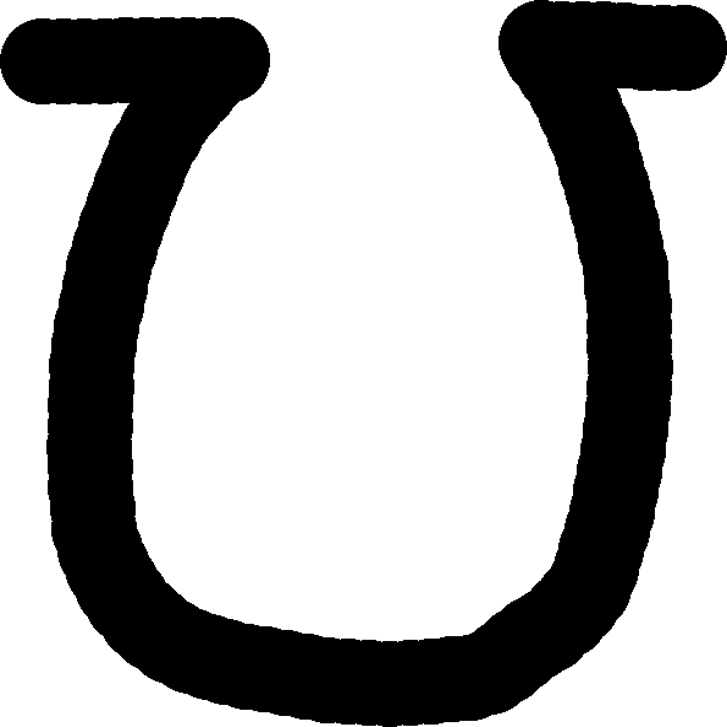
\includegraphics[height = 0.08\textheight]{../assets/images/horseshoe}} ;
	
	\draw[->, very thick] ([yshift = -0.15cm]saddler.west) -- ([yshift = -0.15cm]smith.east) node[midway, below]{
\includegraphics[height = 0.08\textheight]{../assets/images/potatoes}};
	
	\node (farmer) at (0, -2){
\includegraphics[height = 0.15\textheight]{../assets/images/agents/agent_right}};
	\draw[->, very thick] (smith.south east) -- (farmer.north west) node[midway, above right]{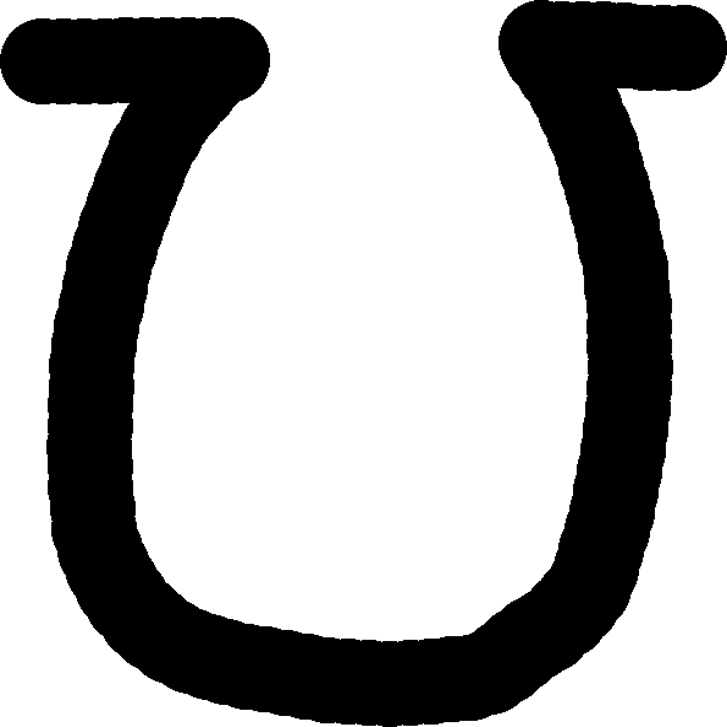
\includegraphics[height = 0.08\textheight]{../assets/images/horseshoe}};
	\draw[<-, very thick] ([xshift = -0.4cm] smith.south east) -- ([xshift = -0.4cm] farmer.north west) node[midway, below left]{
\includegraphics[height = 0.08\textheight]{../assets/images/potatoes}};
	
	\draw[->, very thick] (saddler.south west) -- (farmer.north east) node[midway, above left]{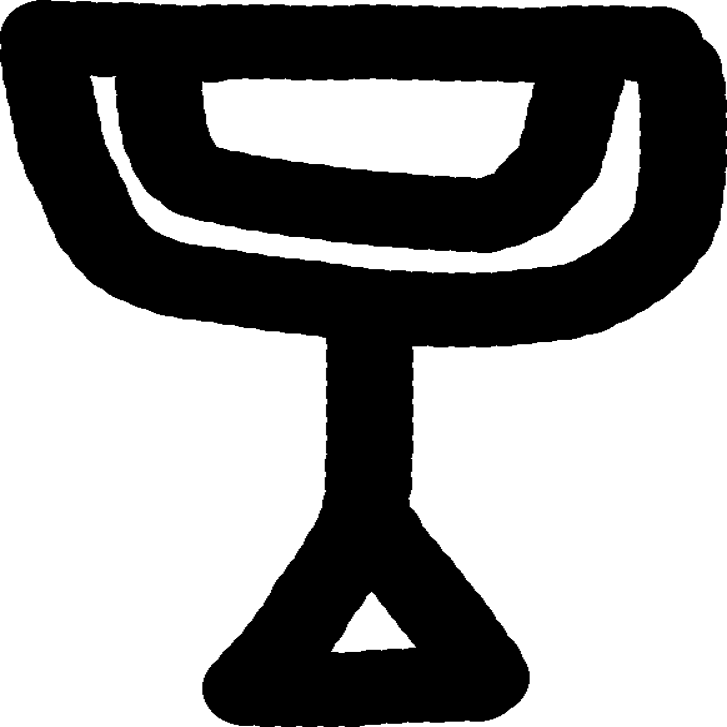
\includegraphics[height = 0.08\textheight]{../assets/images/saddle}};
	\draw[<-, very thick] ([xshift = 0.4cm] saddler.south west) -- ([xshift = 0.4cm] farmer.north east) node[midway, below right]{
\includegraphics[height = 0.08\textheight]{../assets/images/potatoes}};
	
\end{tikzpicture}	
	\end{figure}
\end{frame}
%%%

%%%
\begin{frame}{Dominant Medium of Exchange}
	The probability that I will accept ($\pi$) a good as a medium of exchange depends on my expectations that other people will do the same ($\Pi$).\\
	\vspace{1.5em}
	\uncover<2->{\textbf{Assumptions:} $0 \leq \pi \leq 1$; $0 \leq \Pi \leq 1$; $\frac{\delta U(\pi)}{\delta \Pi} > 0\ \forall \pi > 0$}
\end{frame}
%%%


%%%
\begin{frame}{Dominant Medium of Exchange}
	The acceptance of money as a coordination game:
	\begin{columns}[T]
		\begin{column}{0.5\textwidth}
			\begin{footnotesize}
				\begin{itemize}
					\item \alert<1>{If $\Pi = 0$: choose $\pi = 0$}
					\item<2-> \alert<2>{If $\Pi = 1$: choose $\pi = 1$}
					\item<3-> \alert<3>{If $\Pi > \hat\Pi > 0$: choose $\pi = 1$}
					\item<3-> \alert<3>{If $\Pi < \hat\Pi < 1$: choose $\pi = 0$}
				\end{itemize}
			\end{footnotesize}
			\begin{figure}
				\begin{tikzpicture}

% define positions
\coordinate (0) at (0,0);
\coordinate (1) at (1,1);
\coordinate (2) at (-1,2);
\coordinate (3) at (-2,0);
\coordinate (4) at (-3,1);

% draw economic agent
\node at (4) {
\includegraphics[height = 0.15\textheight]{../assets/images/agents/handing_money_right}};

% last, first and second slide
\alt<3>{
	% NE			
	% expectation of PI > PI_hat > 0: choose pi = 1
	% expectation of PI < PI_hat < 1: choose pi = 0
	\node at (0) {
\includegraphics[height = 0.15\textheight]{../assets/images/agents/nope_left}};
	\node at (1) {
\includegraphics[height = 0.15\textheight]{../assets/images/agents/reaching_left}};
	\node at (2) {
\includegraphics[height = 0.15\textheight]{../assets/images/agents/nope_left}};
	\node at (3) {
\includegraphics[height = 0.15\textheight]{../assets/images/agents/reaching_left}};
}{
	% expectation of PI = 0: choose pi = 0
	\only<1>{
		\node at (0) {
\includegraphics[height = 0.15\textheight]{../assets/images/agents/nope_left}};
		\node at (1) {
\includegraphics[height = 0.15\textheight]{../assets/images/agents/nope_left}};
		\node at (2) {
\includegraphics[height = 0.15\textheight]{../assets/images/agents/nope_left}};
		\node at (3) {
\includegraphics[height = 0.15\textheight]{../assets/images/agents/nope_left}};
	}
	% expectation of PI = 1: choose pi = 1
	\only<2>{
		\node at (0) {
\includegraphics[height = 0.15\textheight]{../assets/images/agents/reaching_left}};
		\node at (1) {
\includegraphics[height = 0.15\textheight]{../assets/images/agents/reaching_left}};
		\node at (2) {
\includegraphics[height = 0.15\textheight]{../assets/images/agents/reaching_left}};
		\node at (3) {
\includegraphics[height = 0.15\textheight]{../assets/images/agents/reaching_left}};
	}
}
\end{tikzpicture}
			\end{figure}
		\end{column}
		\begin{column}{0.5\textwidth}
			\begin{figure}
				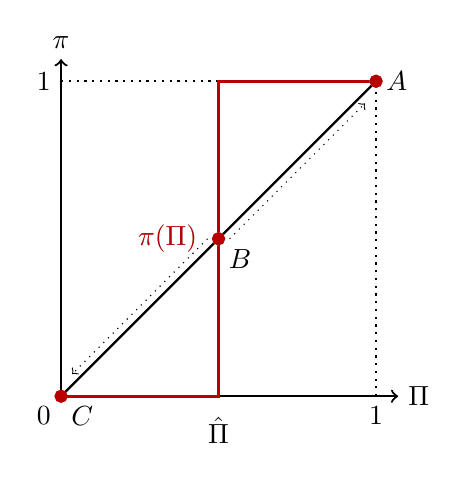
\begin{tikzpicture}[thick]
		
		% define coordinates
			\coordinate[label=below left:$0$] (0) at (0,0);
			\coordinate[label=below:$1$] (1x) at (4,0);
			\coordinate[label=left:$1$] (1y) at (0,4);
			\coordinate (1) at (4,4);
			\coordinate (mid) at (2,2);
			\coordinate (midx) at (2,0);
			\coordinate (midx2) at (2,4);
		
		% draw axes
			\draw[->] (0) -- ([xshift = 8pt] 1x);
			\draw[->] (0) -- ([yshift = 8pt] 1y);
			
		% draw dotted lines
			\draw[dotted] (1y) -- (midx2);
			\draw[dotted] (1x) -- (1);
			
		% draw diagonals
			\draw (0) -- (1);
			\uncover<3->{
				\draw[->, dotted, thin] ([xshift = -4pt] mid) -- ([xshift = 4pt, yshift = 8pt] 0);
				\draw[->, dotted, thin] ([xshift = 4pt] mid) -- ([xshift = -4pt, yshift = -8pt] 1);
			}
		
		% draw NEs
			% line
			\draw[highlight, very thick] (0) -- (midx) -- (midx2) -- (1);
			\uncover<3->{\draw[focus, very thick] (0) -- (midx) -- (midx2) -- (1);}
			
			% A
			\filldraw[focus] (0) circle (2pt);
			\filldraw[highlight] (1) circle (2pt);
			
			% B
			\uncover<2->{\filldraw[focus] (1) circle (2pt);}
			\filldraw[highlight] (mid) circle (2pt);
			\uncover<3->{\filldraw[focus] (mid) circle (2pt);}
								
		% labels
			\node[right] at (1) {$A$};
			\node[below right] at (mid) {$B$};
			\node[below right] at (0) {$C$};
			\node[right = 8pt] at (1x) {$\Pi$};
			\node[above = 8pt] at (1y) {$\pi$};
			\node[above = 24pt, left = 4pt, highlight] at (mid) {$\pi(\Pi)$};
			\uncover<3->{\node[above = 24pt, left = 4pt, focus] at (mid) {$\pi(\Pi)$};}
			\node[below = 4pt] at (midx) {$\hat\Pi$};
			
\end{tikzpicture}
			\end{figure}
		\end{column}
	\end{columns}
\end{frame}
%%%

%%%
\begin{frame}{Medium of Exchange}
	Double coincidence of wants: find someone who has bread \textcolor{focus}{\textbf{and}} wants an apple.
	\begin{columns}
		\begin{column}{0.5\textwidth}
			\begin{figure}
				\begin{center}
					
\includegraphics[height = 0.1\textheight]{../assets/images/bread}
				\end{center}
			\end{figure}
		\end{column}
		\begin{column}{0.5\textwidth}
			\begin{figure}
				\begin{center}
					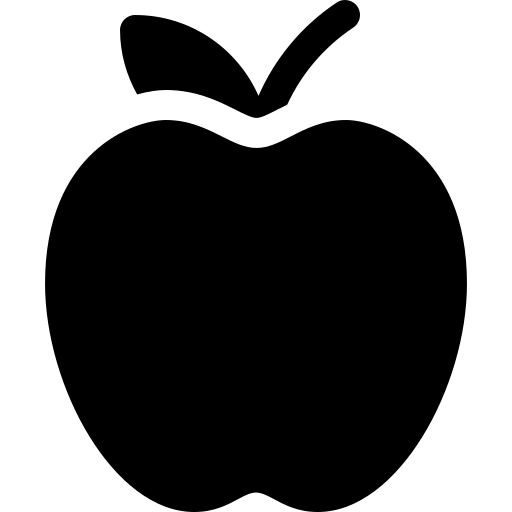
\includegraphics[width = 0.1\textheight]{../assets/images/apple}
				\end{center}
			\end{figure}
		\end{column}
	\end{columns}
	\vspace{1.5em}
	\uncover<2->{Number of trading pairs in a very simple economy:}
	\begin{columns}[T]
		\begin{column}{0.5\textwidth}
			\uncover<2->{
				\begin{scriptsize}
					\begin{center}
						\begin{tabular}{l||c|c|c|c}
			    				& 
\includegraphics[height = 0.05\textheight]{../assets/images/bread} & 
\includegraphics[height = 0.05\textheight]{../assets/images/meat} & 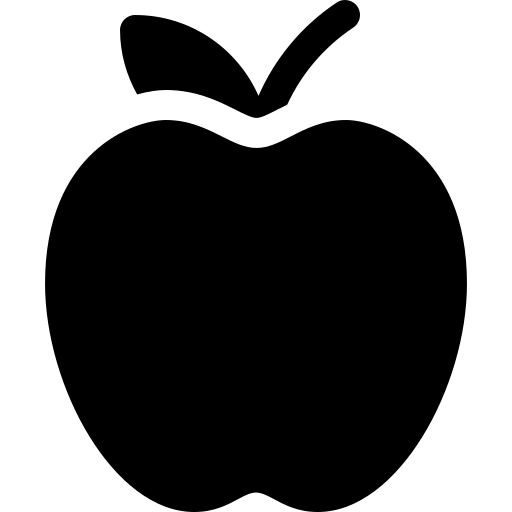
\includegraphics[height = 0.05\textheight]{../assets/images/apple} & 
\includegraphics[height = 0.05\textheight]{../assets/images/potatoes} \\ \hline \hline
							
\includegraphics[height = 0.05\textheight]{../assets/images/bread}    & \cellcolor{black!50} & \cellcolor{highlight!50} & \cellcolor{highlight!50} & \cellcolor{highlight!50} \\ \hline
							
\includegraphics[height = 0.05\textheight]{../assets/images/meat} &      & \cellcolor{black!50} & \cellcolor{highlight!50} & \cellcolor{highlight!50} \\ \hline
							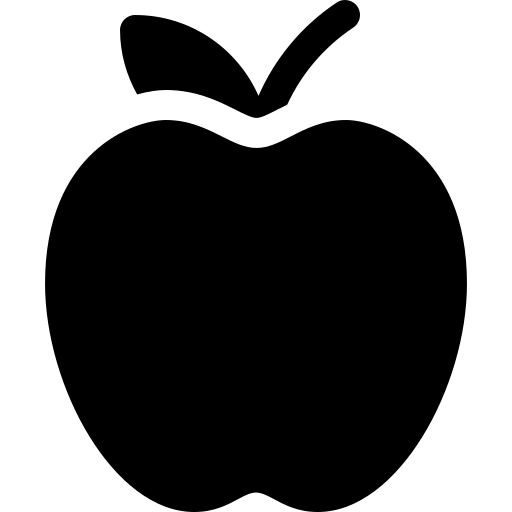
\includegraphics[height = 0.05\textheight]{../assets/images/apple}  &      &         & \cellcolor{black!50} & \cellcolor{highlight!50} \\ \hline
							
\includegraphics[height = 0.05\textheight]{../assets/images/potatoes}    &      &         &        & \cellcolor{black!50} \\
						\end{tabular}
					\end{center}
				\end{scriptsize}
			}
		\uncover<2->{
			\begin{align*}
				\frac{n^2-n}{2} = \frac{n(n-1)}{2}
			\end{align*}
		}
		\end{column}
		\begin{column}{0.5\textwidth}
			\uncover<3->{
				\begin{scriptsize}
					\begin{center}
						\begin{tabular}{l||c|c|c|c}
								& 
\includegraphics[height = 0.05\textheight]{../assets/images/bread} & 
\includegraphics[height = 0.05\textheight]{../assets/images/meat} & 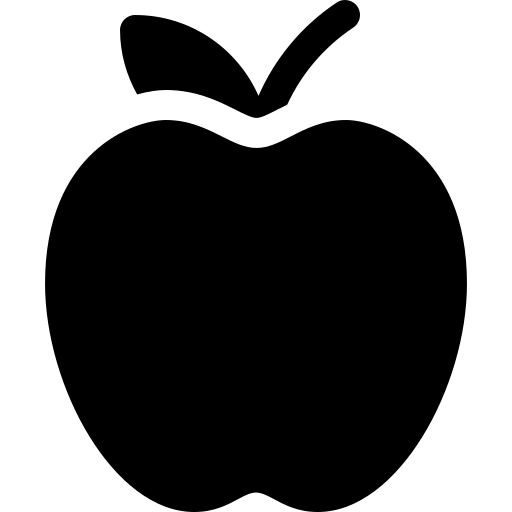
\includegraphics[height = 0.05\textheight]{../assets/images/apple} & 
\includegraphics[height = 0.05\textheight]{../assets/images/potatoes} \\ \hline \hline
							
\includegraphics[height = 0.05\textheight]{../assets/images/potatoes}    &      &         &        & \cellcolor{black!50} \\
						\end{tabular}
					\end{center}
				\end{scriptsize}
				\uncover<3->{
					\vspace{4.5em}
					\begin{align*}
						n-1
					\end{align*}
				}
			}
		\end{column}
	\end{columns}
\end{frame}

%%%

%%%
\begin{frame}{Medium of Exchange}
	\begin{figure}
		\begin{footnotesize}
	\begin{tikzpicture}
		\begin{axis}[xmin = 0, xmax = 16,
						ymin = 0, ymax = 125,
						width = 0.9\textwidth,
						height = 0.7\textheight,
						legend pos = north west,
						xtick distance = 5,
						ytick distance = 50,
						grid = both,
						xlabel = {Number of goods and services $n$},
						ylabel = {Possible pairs of trading goods}
						]
					
			\addplot[focus, domain = 0:16, very thick] {(x^2 - x) / 2};
			\addplot[highlight, domain = 0:16, very thick] {x - 1};
		
			\legend{
				Without money, 
				With money
			};
		\end{axis}
	\end{tikzpicture}
\end{footnotesize}
	\end{figure}
\end{frame}
%%%


%%%
\begin{frame}{Examples of Dominant Media of Exchange}
	\begin{figure}
		\begin{tikzpicture}[scale = 0.8]
	\begin{footnotesize}
		\coordinate (1) at (-4, 3);
		\coordinate (2) at (0, 3);
		\coordinate (3) at (4, 3);
		\coordinate (4) at (-4, 0);
		\coordinate (5) at (0, 0);
		\coordinate (6) at (4, 0);

		\node at (1) {\begin{tikzpicture}
	\node[circle, fill = black, scale = 2.5] (stone) at (0,0) {};
	\node[circle, fill = white, scale = 0.5] (hole) at (0,0) {};
	
	\node[circle, draw, scale = 2.5] (ring) at (0.01, 0.01) {};
	\node[circle, draw, scale = 0.5] (ring2) at (0.01, 0.01) {};
\end{tikzpicture}};
		\node[below = 12pt] at (1) {Millstones on Yap};
	
		\node at (2) {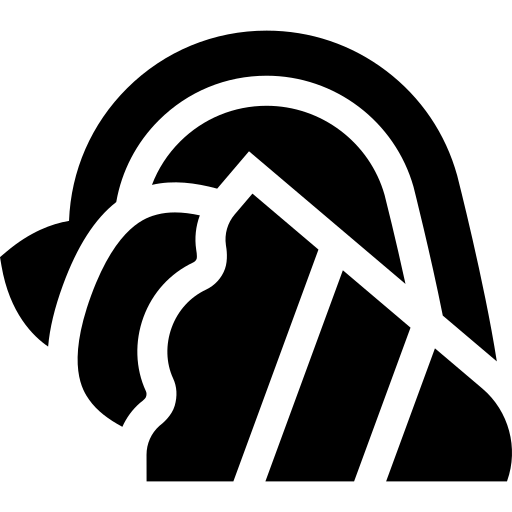
\includegraphics[height = 0.1\textheight]{../assets/images/shell}};
		\node[below = 12pt] at (2) {Shells};

		\node at (3) {
\includegraphics[height = 0.1\textheight]{../assets/images/cigarettes}};
		\node[below = 12pt] at (3) {Cigarettes};

		\node at (4) {
\includegraphics[height = 0.1\textheight]{../assets/images/jewel}};
		\node[below = 12pt] at (4) {Jewellery};

		\node at (5) {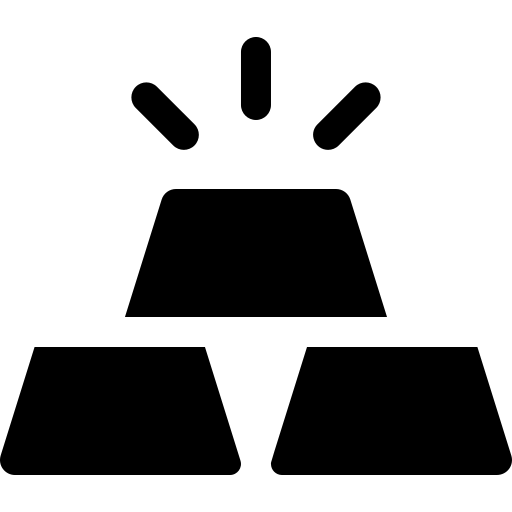
\includegraphics[height = 0.1\textheight]{../assets/images/ingots}};
		\node[below = 12pt] at (5) {Metal money};

		\node at (6) {
\includegraphics[height = 0.1\textheight]{../assets/images/currency}};
		\node[below = 12pt] at (6) {Currency};

	\end{footnotesize}
\end{tikzpicture}	
	\end{figure}
\end{frame}
%%%

%%%
\begin{frame}{Unit of Account}
	The same problem occurs for the quantity ratios:
	\vspace{1em}
	\begin{center}
		\begin{tabular}{l||c|c|c|c}
       			& 
\includegraphics[height = 0.05\textheight]{../assets/images/bread} & \includegraphics[height = 0.05\textheight]{../assets/images/meat} & \includegraphics[height = 0.05\textheight]{../assets/images/apple} & \includegraphics[height = 0.05\textheight]{../assets/images/potatoes} \\ \hline \hline
			\includegraphics[height = 0.05\textheight]{../assets/images/bread}    & 1:1 & \cellcolor{highlight!50} & \cellcolor{highlight!50} & \cellcolor{highlight!50} \\ \hline
			\includegraphics[height = 0.05\textheight]{../assets/images/meat} &   1:8   & 1:1 & \cellcolor{highlight!50} & \cellcolor{highlight!50} \\ \hline
			\includegraphics[height = 0.05\textheight]{../assets/images/apple}  &   1:2  &    4:1 & 1:1 & \cellcolor{highlight!50} \\ \hline
			\includegraphics[height = 0.05\textheight]{../assets/images/potatoes}    &   1:4  &    2:1  &  1:2    & 1:1     
		\end{tabular}
	\end{center}
	\vspace{1.5em}
	\uncover<2->{
		Instead, describe the price in terms of the dominant medium of exchange:\\
		\begin{itemize}
			\item Bread = 0.25 potato 
			\item Meat = 2 potato
			\item Apple = 0.5 potato
		\end{itemize}
	}
\end{frame}
%%%

%%%
\begin{frame}{Store of Value}
	Why do people save?
	\begin{columns}[T]
		\begin{column}{0.5\textwidth}
			\begin{figure}
				\includegraphics[height = 0.1\textheight]{../assets/images/cake}
			\end{figure}
		\end{column}
		\begin{column}{0.5\textwidth}
			\begin{figure}
				\uncover<2->{\includegraphics[height = 0.1\textheight]{../assets/images/mansion}}
			\end{figure}
		\end{column}
	\end{columns}
	\uncover<3->{
		\begin{figure}
			\begin{footnotesize}
	\alt<4>{
	\begin{tikzpicture}
			\begin{axis}[
				xmin = 1959, xmax = 2019, xlabel = Time, /pgf/number format/1000 sep={},
				ymin = 0, ymax = 1, ylabel = {Real value of money, 1960 = 1},
				height = 5cm,
				width = 11cm,
				grid = both,
				legend pos = south west
				]
				\addplot[thick] table[x=time, y=usa, col sep=comma] {../assets/data/cpi.csv};
				\addplot[thick, focus] table[x=time, y=gbp, col sep=comma] {../assets/data/cpi.csv};
				\addplot[thick, highlight] table[x=time, y=swi, col sep=comma] {../assets/data/cpi.csv};
				\addplot[thick, dotted] table[x=time, y=jpy, col sep=comma] {../assets/data/cpi.csv};
	
				\legend{
					USD, 
					GBP,
					CHF,
					JPY
				};
			\end{axis}
		\end{tikzpicture}
	}{
		\begin{tikzpicture}
			\begin{axis}[
				xmin = 1959, xmax = 2019, xlabel = Time, /pgf/number format/1000 sep={},
				ymin = 10^(-15), ymax = 1, ylabel = {Real value of money, 1960 = 1}, ymode = log,
				height = 5cm,
				width = 11cm,
				grid = both,
				legend pos = south west
				]
				\addplot[thick] table[x=time, y=arg, col sep=comma] {../assets/data/cpi.csv};
				\addplot[thick, focus] table[x=time, y=mex, col sep=comma] {../assets/data/cpi.csv};
				\addplot[thick, highlight] table[x=time, y=tur, col sep=comma] {../assets/data/cpi.csv};
	
				\legend{
					ARS, 
					MXN,
					TRY
				};
			\end{axis}
		\end{tikzpicture}
	}
\end{footnotesize}
			\caption*{\textit{Data}: FRED Economic Research}
		\end{figure}
	}
\end{frame}
%%%

%%%
\begin{frame}{The Properties of Money}	
	\begin{figure}
		\begin{tikzpicture}[scale = 0.8]
	\begin{footnotesize}
		
		\coordinate (1) at (-4, 3);
		\coordinate (2) at (0, 3);
		\coordinate (3) at (4, 3);
		\coordinate (4) at (-4, 0);
		\coordinate (5) at (0, 0);
		\coordinate (6) at (4, 0);
		\coordinate (7) at (0, -3);

			
		\node at (1) {\includegraphics[height = 0.1\textheight]{../assets/images/rotten_apple}};
		\node[below = 12pt] at (1) {Storability};
		
		\uncover<2->{
			\node[minimum size = 0.35cm] at (2) {\begin{tikzpicture}
	\node[circle, fill = black, scale = 2.5] (stone) at (0,0) {};
	\node[circle, fill = white, scale = 0.5] (hole) at (0,0) {};
	
	\node[circle, draw, scale = 2.5] (ring) at (0.01, 0.01) {};
	\node[circle, draw, scale = 0.5] (ring2) at (0.01, 0.01) {};
\end{tikzpicture}};
			\node[below = 12pt] at (2) {Transferability};
		}
		
		\uncover<3->{
			\node at (3) {\includegraphics[height = 0.1\textheight]{../assets/images/ingots}};
			\node[below = 12pt] at (3) {Divisibility};
		}
		
		\uncover<4->{
			\node at (4) {\includegraphics[height = 0.1\textheight]{../assets/images/car}};
			\node[below = 12pt] at (4) {Fungibility};
		}
		
		\uncover<5->{
			\node at (5) {\includegraphics[height = 0.1\textheight]{../assets/images/check}};
			\node[below = 12pt] at (5) {Verifiability};
		}
		
		\uncover<6->{
			\node at (6) {\includegraphics[height = 0.1\textheight]{../assets/images/sand}};
			\node[below = 12pt] at (6) {Scarcity};
		}
		
		\uncover<7->{
			\node at (7) {\includegraphics[height = 0.1\textheight]{../assets/images/wheat}};
			\node[below = 12pt] at (7) {Low Price Volatility};
		}
		
	\end{footnotesize}
\end{tikzpicture}	
	\end{figure}
\end{frame}
%%%

%%%
\begin{frame}{Monetary Value}
	\begin{table}[h]
		\begin{center}
			\begin{tabular}{rl}
			\hline \hline
  				& \text{Intrinsic value}               \\
			\uncover<2->{\text{+} & \text{Promise of payment}} \\
			\uncover<3->{\text{+} & \text{Liquidity premium}} \\
			\hline
			\uncover<3->{\text{=} & \text{Market value of monetary unit}} \\ \hline \hline
			\end{tabular}
		\end{center}
	\end{table}
	\vspace{0.8cm}
	\textbf{Intrinsic value:} Material value of the good which does not depend on the good's monetary function.\\
	\vspace{0.5em}
	\uncover<2->{\textbf{Promise of payment:} Components which do not depend on the materialistic value of the good. Subject to issuer risk.} \\
	\vspace{0.5em}
	\uncover<3->{\textbf{Liquidity premium:} Option to flexibly trade the monetary unit for arbitrary goods.} \\
	\vspace{0.5em}
%	\uncover<5->{\textbf{Speculation value:} Option of profit in case of increase in value.}
\end{frame}
%%%

%%%
\begin{frame}{Different Types of Money}
	\begin{figure}
		\begin{tikzpicture}[scale = 0.8]
	\begin{footnotesize}
		\draw[dotted] (-5.9, 0) rectangle (-2.1, 4) node[above = 1cm, midway] {\textbf{Commodity money}};
		\draw[dotted] (-1.9, 0) rectangle (1.9, 4) node[above = 1cm, midway] {\textbf{Credit money}};
		\draw[dotted] (2.1, 0) rectangle (5.9, 4) node[above = 1cm, midway] {\textbf{Fiat money}};

		\node at (-5, 2.5) {\includegraphics[height = 0.07\textheight]{../assets/images/shell}};
		\node at (-3, 2.5) {\includegraphics[height = 0.07\textheight]{../assets/images/ingots}};
		\node at (-5, 1) {\includegraphics[height = 0.07\textheight]{../assets/images/jewel}};
		\node at (-3, 1) {\includegraphics[height = 0.07\textheight]{../assets/images/cigarettes}};
		
		\uncover<2->{
			\node[rectangle, thick, draw] at (0, 2.5) {IOU};
		}
		
		\uncover<3->{
			\node at (4, 2.5) {\includegraphics[height = 0.07\textheight]{../assets/images/bulb}};
		}
\end{footnotesize}
\end{tikzpicture}
	\end{figure}
	\vspace{1.em}
	\begin{table}[h]
		\begin{center}
			\begin{tabular}{lccc}
				\hline \hline
					& Intrinsic & Promise & Premium \\
				Commodity money  &   +  &   & (+) \\
				\uncover<2->{Credit money &      & + & (+)} \\
				\uncover<3->{Fiat money  &      &   &  +}  \\ \hline \hline
			\end{tabular}
		\end{center}
	\end{table}
\end{frame}
%%%

\begin{frame}%[allowframebreaks]
\frametitle{References}
	\bibliographystyle{amsplain}
	\bibliography{../assets/bib/refs}
\end{frame}

\end{document}